% Dokumentation Exposé zur Bachelorarbeit
% von Andreas Lorer
% 2015
% Studiengang: Angewandte Informatik - HS Ravensburg-Weingarten
\documentclass[a4paper,11pt,singlespacing]{article}
\usepackage[left=2.5cm,right=2.5cm,top=2.5cm]{geometry}
\usepackage[hyphens]{url}
\usepackage[backend=biber,style=alphabetic,backref=true,citecounter=true,citestyle=authoryear]{biblatex}
\usepackage{csquotes}
\usepackage{hyperref}
\usepackage{setspace}
\usepackage[utf8]{inputenc}
\usepackage[T1]{fontenc}
\usepackage[ngerman]{babel}
\usepackage{color}
\usepackage{hyperref}
\usepackage{pdflscape}
\usepackage{graphicx}
\usepackage{listings}
\usepackage{csquotes}
\addbibresource{zitate.bib}
\pagestyle{myheadings}
\markright{\centerline{Exposé zur Bachelorarbeit}}
\author{Andreas Lorer}

\graphicspath{{images/}}            
\setlength{\parindent}{0ex}         			% Absatzeinrueckung verhindern

\newcommand{\headline}{Exposé zur Bachelorarbeit}
\newcommand{\subheadline}{Webperformance für den mobilen Endanwender}

\begin{document}
	% document styles for listings
	\lstset{
		%numbers=left,
		basicstyle=\ttfamily,
		language=bash,
		keywordstyle=\color{blue},
		commentstyle=\color{green},
		xleftmargin=0.5cm
	}

% Deckblatt
		\begin{center}
			\thispagestyle{empty}
			\vspace{5.0cm}
	    {\large \bfseries \headline}\\[0.5cm]
	    \vspace{2.0cm}
	    {\huge \bfseries \subheadline}\\[1.5cm]
			\vspace{10.0cm}		
		\end{center}


	% Authoren
	  \begin{flushleft}\large
	  \hspace*{2cm} \emph{Autor:}\\
	  \hspace*{2cm} Andreas Lorer | 22652\\
	  \hspace*{2cm} \href{mailto:andreas.lorer@hs-weingarten.de}{\nolinkurl{andreas.lorer@hs-weingarten.de} }\\
	    \hspace*{2cm} 88250 Weingarten\\
	    \hspace*{2cm} Wilhelmstraße 4
	  \end{flushleft}
  	\pagebreak

%Inhaltsverzeichnis
	\tableofcontents 											
	\thispagestyle{empty}
	\pagebreak

\section{Einleitung} % (fold)
\label{sec:einleitung}
	Webperformance ist oft ein stark vernachlässigter Teil der Web- und Anwendungsentwicklung. Viele Anwender empfinden das Internet als sehr langsam.
	\begin{figure}[htbp]
		\begin{center}
			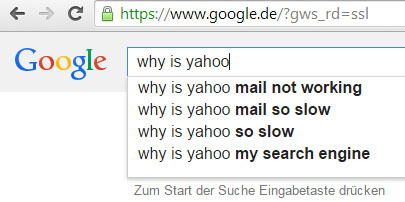
\includegraphics[width=0.5\textwidth]{yahoo.jpg}
		\end{center}
		\caption{Why is Yahoo so slow?}
		\label{fig:YahooIsSlow}
	\end{figure}
	Sucht man bei der Suchmaschine Google nach dem Begriff: "`Why is Yahoo so..."' bekommt man unter den Top vier der Suchanfragen den Vorschlag "`slow"'. Dies trifft auch auf Seiten wie Ebay, Youtube oder Reddit zu. Nicht nur kleine Webseiten, sondern auch große Plattformen haben ein Problem mit Webperformance oder werden zumindest von deren Nutzern so Wahrgenommen. Warum wird also das Internet generell als langsam empfunden?
	\begin{figure}[htbp]
	 	\begin{center}
	 		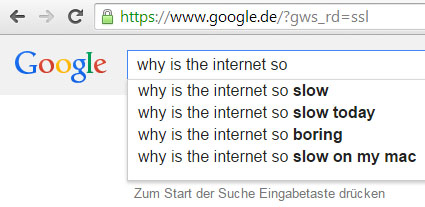
\includegraphics[width=0.5\textwidth]{internet.jpg}
	 	\end{center}
	 	\caption{Why is the Internet so slow?}
	 	\label{fig:internetIsSlow}
	 \end{figure} 

	Das hat sehr viele Gründe. So ist die Geschwindigkeit einer Webseite auf den ersten Blick nicht sichtbar und Kunden zahlen vor allem gerne für Dinge, die für sie greifbar sind. Eine auf Geschwindigkeit optimierte Seite stellt zudem auch einen Mehraufwand dar, den nicht jeder Kunde bezahlen möchte oder es wird von ihm als nicht wichtig angesehen.\\
	Auch die Infrastruktur spielt eine entscheidende Rolle. So ist ein langsamer Seitenaufbau vorranging von der Latenz abhängig, die zwischen dem Anwender und dem Servers besteht.\\
	Zahlen, Fakten und Entwicklungstrends bestätigen, dass Webperformance einen sehr wichtigen Aspekt darstellt und vor allem in der Zukunft eine immer wichtigere Rolle spielen wird.\\
% section einleitung (end)


\section{Motivation} % (fold)
\label{sec:motivation}
	Webperformance ist und wird immer wichtiger.
	Die Nutzung von Mobilen Endgeräten ist in den letzten Jahren stark gewachsen. Zwischen 2011 und 2014 stieg die Anzahl der Smartphone Nutzer von 18\% auf 50\% an. Dies ist ein Wachstum von 32\% innerhalb von 3 Jahren.\autocite{tns14}
	\begin{figure}[htbp]
		\begin{center}
			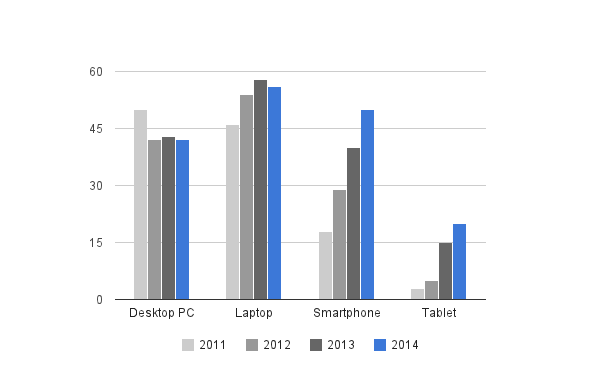
\includegraphics[width=0.9\textwidth]{smartphoneUsage.png}
		\end{center}
		\caption{Gerätenutzung in der Gesamtbevölkerung (2011 – 2014)\autocite{tns14}}
		\label{fig:geraetenutzung}
	\end{figure}
	Das bedeutet, dass immer mehr Nutzer auf Webseiten zugreifen, die entweder erst gar nicht für den Mobilen Anwender optimiert sind (kein Repsonsive-Webdesign) oder die zwar Responsive sind, aber deren Ladezeit und Ladelast so hoch sind, das die Nutzbarkeit der Seite stark eingeschränkt ist. Vor allem im E-Commerce ist Geschwindigkeit ein entscheidender Faktor, ob ein Besucher die Seite bei zu langem Laden verlässt und im schlimmsten Fall auf ein Angebot der Konkurrenz verwendet. Eine Untersuchung von Radware.com hat ergeben:\\

	"`Two out of three mobile shoppers expect pages to load in 4 seconds or less."'\autocite{radware13}\\

	Dabei haben im Schnitt Webseiten die nicht für Mobile optimiert sind eine durchschnittliche Ladezeit von 7.84 Sekunden und Webseiten die für Mobile optimiert sind fallen mit 4.33 Sekunden auch über die 4 Sekunden Marke.\autocite{radware13} 

	Auch Google findet, dass Webperformance wichtig ist und den Anwender glücklicher und zufriedener macht und veröffentlichte bereits 2010, dass Webperformance in das Suchranking mit einfließt:\\

	"`Faster sites create happy users and we've seen in our internal studies that when a site responds slowly, visitors spend less time there. [...] Recent data shows that improving site speed also reduces operating costs. Like us, our users place a lot of value in speed — that's why we've decided to take site speed into account in our search rankings"'\autocite{google10}\\

	Es gibt noch weitere Gründe, warum es wichtig ist, auf Geschwindigkeit als Feature zu setzen. Dies soll in der Bachelorarbeit tiefer aufgeführt werden.
% section motivation (end)


\section{Stand der Forschung} % (fold)
\label{sec:stand_der_forschung}
	Es gibt momentan eine große Anzahl an Maßnahmen die ergriffen werden können, um eine Webseite auf ihre Performance zu optimieren. Sowohl Clientseitig als auch für den Server gibt es viele "`Best-Practices"', Tools oder Plugins, die die Performance erhöhen. Viele der "`Best-Practices"' stellen sich aber momentan als "`Workaround"' für das 20 Jahre alte HTTP/1.1 Protokoll heraus. In der Zukunft wird dieses Protokoll von HTTP/2.0 abgelöst werden, was viele Verbesserungen mit sich bringen wird die momentan noch sehr umständlich manuell gelöst werden müssen.
% section stand_der_forschung (end)



\section{Zielsetzung} % (fold)
\label{sec:zielsetzung}
	Die Bachelorarbeit soll einen Überblick über die heute gängigen Methoden zur Verbesserung der Webperformance schaffen. Es sollen "`Best-Practices"' gefunden und vorgestellt werden, Pattern und Anti-Pattern diskutiert und im Praktischen Teil der Arbeit soll eine Webseite mit einer Bildergalerie entstehen, die in möglichst kurzer Zeit (< 2 Sekunden) auf dem Smartphone lädt.
% section zielsetzung (end)



\section{Bedeutung der Arbeit} % (fold)
\label{sec:bedeutung_der_arbeit}
	Die Arbeit soll untersuchen, welche Auswirkungen die verschiedenen Methoden auf die Ladezeit einer Seite haben. Es soll herausgearbeitet werden, wie ein optimaler "`Workflow"' aussehen könnte und wie dieser bereits bei Projektstart eingesetzt werden kann. Das soll ermöglichen Projekte zu verwirklichen die bereits bei der Entwicklung performant sind und nicht erst am Schluss an der Performance nachgearbeitet werden muss. 
% section bedeutung_der_arbeit (end)



\section{Gliederung} % (fold)
\label{sec:gliederung}

	\subsection{Abstract} % (fold)
	\label{sub:abstract}
	% subsection abstract (end)

	\subsection{Probjektbeschreibung}
	\label{sub:probjektbeschreibung}
		\begin{itemize}
			\item Problem beschreiben: Warum ist das Internet vor allem auf Mobile Devices langsam?
			\item Motivation: Google rankt Performante Seiten höher. First visitors bleiben auf der Seite ect...
			\item Features
			\item Zielgruppe
			\item Fähigkeiten der Nutzer?
			\item Eingrenzung des Themas: Was wird behandelt und was nicht?
			\item Zielsetzung: Schnell: "First-Render" nach unter 2 Sekunde von einem Deutschen Server (Messbarkeit).
			Best Practices, Methoden, Schranken / Grenzen
			\item "`Ist-Zustand:"' Webperformance wird nicht als sehr wichtiges Feature angesehen. Punkte dafür finden was dafür Spricht. Negative Aspekte aufgreifen und vorweg nehmen. Argumente für Webperformance aufführen.
			\item "`Soll-Zustand:"' Workflow und Best-Practices die bereits bei Projekt beginn eingesetzt werden können.
		\end{itemize}
	% subsection probjektbeschreibung (end)


	\subsection{Grundlagen}
	\label{sub:grundlagen}
		\begin{itemize}
			\item Begriffe (Above the Fold, Critical Render Path, Payload, TTFB, RTT)
			\item Tools (pro / contra)
			\item Latenz \& Netze
			\item Http/1.1
			\item Datenvolumen / Datenrate (Steigende anz. an Bildern)
		\end{itemize}


			\subsubsection{Prozess der Suche}
			\label{sub:prozess_der_suche}
				\begin{itemize}
					\item Auf welche Frage suche ich eine Antwort? -> was gibt es momentan für Methoden und welche davon sind für mich einsetzbar?
					\item  Was habe ich gefunden? Was ist daran gut / schlecht und was gibt es für alternativen?
					\item Warum verwende ich XY und nicht AB?
				\end{itemize}
			% subsection prozess_der_suche (end)
	% subsection grundlagen (end)


	\subsection{Entwicklung}
	\label{sub:entwicklung}
		\begin{itemize}
			\item Was hat die Abteilung bereits Entwickelt?
			\item Baut es auf etwas Bestehendem auf?
			\item Was soll am Ende des Projekts rauskommen?
			\item Vorgehensweise
			\item Entwicklungsverlauf (Messungen, Daten, Analyse, Folgerungen)
		\end{itemize}
	% subsection _entwicklung_ (end)


	\subsection{Prozess der Validierung}
	\label{sub:prozess_der_validierung}
		\begin{itemize}
			\item Wie überprüfe ich den Erfolg des Projektes? Diagramme? Flow-Charts? Zahlen, Fakten ect...
			\item Was ist in der Praxis durchsetzbar und was nicht?
			\item Was ist in diesem Projekt vielleicht möglich aber sonst generell nicht? Wo sind die Schranken? 
			\item Was sind meine Erkenntnisse? Neue?
			\item Was hat sich zum "Ist"-Zustand geändert und was nicht?
			\item Ist das Projekt abgeschlossen? Was ist der Stand?
		\end{itemize}
	% subsection prozess_der_validierung (end)


	\subsection{Zusammenfasssung}
	\label{sub:zusammenfasssung}
		Erkentnisse (best-practices): Auflistung aller Performance möglichkeiten unterteilt in Server / Client / Workflow / Programming / Tools.\\

		\subsubsection{Workflow \& Programming} % (fold)
		\label{ssub:workflow_programming}
		\begin{itemize}
			\item Performance durch performanten Code
			\item Dom Manipulation bei onload vermeiden
			\item Loops vermeiden
			\item Concatenating von files (Achtung: load and execute order!!)
			\item Uglyfy / Minify code
			\item Libraries / Frameworks wirklich benötigt
			\item Bootstrap customize
			\item (optional) Was für Programmcode braucht mehr Leistung als anderer bei dem selben Ergebnis? (Stichwort: Eventlistener, Event-Delegation, Event-Bubbling)
		\end{itemize}
	% subsubsection workflow_programming (end)
	

		\subsubsection{Server} % (fold)
		\label{ssub:server}
		\begin{itemize}
			\item DNS lookups
			\item Caching von statischen elementen (beachte: how to override cached files for clients)
			\item Server side rendering vs client side (siehe zitate: twitter)
			\item ModPageSpeed Apache / Nginx Plugin
		\end{itemize}	
		% subsubsection server (end)
		

		\subsubsection{Client} % (fold)
		\label{ssub:client}
		\begin{itemize}
			\item Critical Render path, 
			\item Render blocking javascript, 
			\item above the fold
			\item Lazy loading
			\item Schlaue request? / Ajax loading
			\item inline css and scripts vs External scripts
			\item Image format webp / jpg pros (30\% kleiner) and cons (nicht supported)
			\item (<img srcset="...")
			\item Image optimierung (save as../ save for web), Progressive Images, Scaling usw.
			\item Browser caching, allgemeines caching
		\end{itemize}
		% subsubsection client (end)

		\subsubsection{Best Practices} % (fold)
		\label{ssub:best_practices}
			\begin{itemize}
				\item Einschränkungen (shared hosts / kein root-Zugang ect.)
				\item Patterns und Anti-Pattern
				\item Methoden
				\item Ausblick (HTTP/2.0, responsive img-Tag)
			\end{itemize}
		% subsubsection best_practices (end)
	% subsection zusammenfasssung (end)
% section gliederung (end)

\section{Vorgehen} % (fold)
\label{sec:vorgehen}
	Eine bereits in ihren Grundgerüst bestehende Bildergallery soll als "`Dummy-Projekt"' benutzt werden um zu testen, anzuwenden und messbar zu machen. Die daraus resultierenden Erkenntnisse sollen in der Arbeit ausgewertet und bewertet werden. 
% section vorgehen (end)

\section{Herausforderungen} % (fold)
\label{sec:herausforderungen}
	Eine Herausforderung wird sein, das Projekt auf einem Server aufzusetzen auf dem ich mit \texttt{Root-Rechten} zugreifen kann und diesen mit den entsprechenden Plugins und Einstellungen zu konfigurieren. Hier kommt entweder der Cloudcomputing-Service von Amazon (AWS - Amazon Web Services) oder Microsoft (Azure) in Frage. Vor allem meine geringen Kentnisse in diesem bereich macht es sehr schwer Abschätzbar wieviel Aufwand und Einarbeitungszeit hier benötigt werden.\\
	Es wird Schwierigkeiten geben die angewendeten Methoden zur Performance Steigerung Messbar zu machen und darzustellen. \\
	Zudem wird es eine Herausforderung sein, die Webseite so zu verbessern, dass sie in weniger als 2 Sekunden Ladet. 
% section herausforderungen (end)

\section{Zeitplan} % (fold)
\label{sec:zeitplan}
	1. Meilenstein: Setup
	\begin{itemize}
		\item Outline der Arbeit erstellen
		\item Anmeldung der Arbeit
		\item Aufsetzen des Projekts Lokal und auf einem der unter \ref{sec:herausforderungen} aufgelisteten Webservices.
		\item Automatisierte Messung der Ladezeiten einer Webseite einrichten (webpagetest API)
	\end{itemize}

	2. Meilenstein: Performance Tuning
	\begin{itemize}
		\item Recherche nach Performance Methoden
		\item Implementierung der gängigen Practices
		\item Performance Tuning der bestehenden Bildergallery
	\end{itemize}

	3. Meilenstein: Auswertung der Messdaten
	\begin{itemize}
		\item Archivierung
		\item Verbildlichung
		\item Strukturierung des Materials für den Schriftlichen Teil
		\item Treffen mit Betreuer
	\end{itemize}

	4. Meilenstein: Schreiben der Arbeit
	\begin{itemize}
		\item Quellen zu den einzelnen Punkten strukturieren
		\item Reinschrift
		\item Korrekturen
		\item Treffen mit Betreuer
		\item Korrekturen
		\item Abgabe der Arbeit
	\end{itemize}

% section zeitplan (end)

\pagebreak
\printbibliography

\end{document}